\begin{figure}[H]
    \centering
    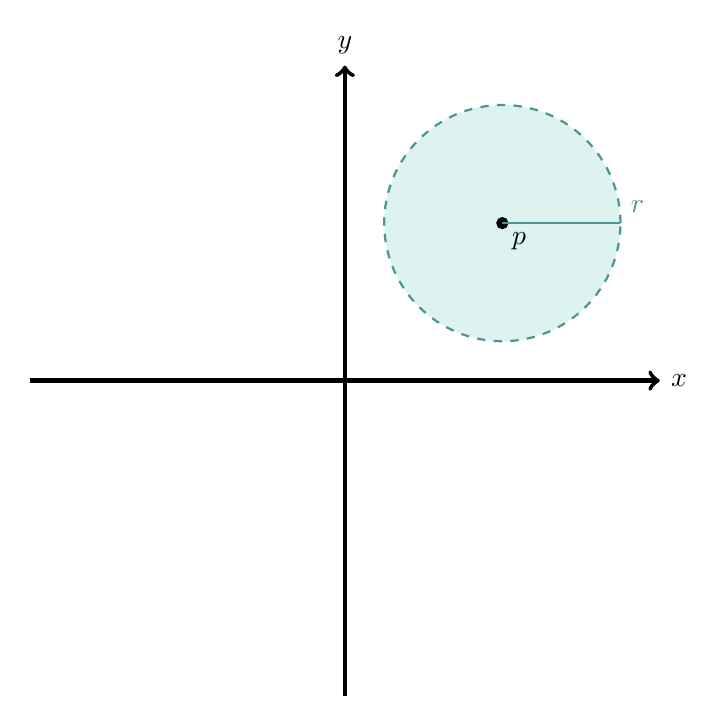
\begin{tikzpicture}
        % Bola aberta.
        \path[fill=BlueGreen!16] (2,2) circle (1.5);
        \draw[BlueGreen!70!black, dashed, thick] (2,2) circle (1.5);

        \draw[->,ultra thick] (-4,0)--(4,0) node[right]{$x$};
        \draw[->,ultra thick] (0,-4)--(0,4) node[above]{$y$};

        % Centro da bola.
        \filldraw[black] (2,2) circle (2pt);
        \node[below right] at (2,2) {$p$};

        % Desenho do raio da bola.
        \draw[BlueGreen!70!black, thick] (2,2) -- (3.5,2) node[above right]{$r$};
    \end{tikzpicture}
    \caption{Bola aberta de centro $p$ e raio $r$ em $\mathbb R^2$.}
    \label{fig:bolaAbertaR2}
\end{figure}
